% --- SLIDE 16: The Challenge and The Core Idea ---
% \begin{frame}{The Challenge: Storing Path Information}
%     \framesubtitle{$\mathcal{O}$-Sets Can Be Huge!}

%     \begin{itemize}
%         \item \textbf{Problem}: The size $|\mathcal{O}_v|$ can grow very large!
%         \item \textbf{Question:} Can we represent the necessary information more compactly?
%     \end{itemize}

%     \begin{alertblock}<2->{Core Idea: Partitioning + Indirection}
%         \begin{enumerate}
%             \item<2-> Partition vertices $V$ into:
%                 \begin{itemize}
%                     \item \textbf{Explicit Vertices ($V_E$):} Typically sinks. Store their $\mathcal{O}_v$ directly.
%                     \item \textbf{Implicit Vertices ($V_I$):} All others. Do \emph{not} store $\mathcal{O}_v$ directly.
%                 \end{itemize}
%             \item<3-> For implicit $v \in V_I$, reconstruct $\mathcal{O}_v$ on-the-fly using:
%                 \begin{itemize}
%                     \item A chosen \textbf{designated successor} $\sigma(v) \in Succ(v)$.
%                     \item An \textbf{offset sequence} $\mathcal{J}_v$ stored at $v$.
%                 \end{itemize}
%         \end{enumerate}
%     \end{alertblock}

% \end{frame}


\begin{frame}{The Challenge: Storing Path Information}
    \framesubtitle{$\mathcal{O}$-Sets Can Be Huge!}

    % Problema e Domanda rimangono uguali
    \begin{itemize}
        \item \textbf{Problem}: The size $|\mathcal{O}_v|$ can grow very large!
        \item \textbf{Question:} Can we represent the necessary information more compactly?
    \end{itemize}


    \begin{alertblock}<2->{Core Idea: Partitioning + Indirection}
        Partition vertices $V$ into two types:
    \end{alertblock}
    \vspace{-1em}
    \begin{columns}[T] % T allinea al top
        \begin{column}{0.48\textwidth}
            \begin{block}<2->{1. Explicit Vertices ($V_E$)}
                \centering
                Store $\mathcal{O}_v$ directly. \\
                (\textit{Simple, but potentially large})
            \end{block}
            % \uncover<3->{\textbf{}
        \end{column}

        \begin{column}{0.48\textwidth}
            \begin{block}<2->{2. Implicit Vertices ($V_I$)}
                \centering
                Do \emph{not} store $\mathcal{O}_v$ explicitly \\
                (\textit{Reconstruct on-the-fly.})
            \end{block}
            \vspace{0.5em}
        \end{column}
    \end{columns}
    \uncover<3->{\textbf{Reconstruction for $v \in V_I$ using}:
        \begin{itemize}
            \item Designated Successor $\sigma(v)$
            \item Offset Sequence $\mathcal{J}_v$ (at $v$)
        \end{itemize}
    }
\end{frame}



% --- SLIDE 17: Successor Choice and Offset Sequence ---
\begin{frame}{Implicit Reconstruction: Successor \& Offset}
    \framesubtitle{How $V_I$ Nodes Refer to Others}

    \begin{block}{1. Designated Successor $\sigma(v)$ (for $v \in V_I$)}
        Which successor should $v$ point to?
        \textbf{Heuristic}: Choose $u = \sigma(v)$ that minimizes $|\mathcal{O}_u|$.
        \[ \sigma(v) \in \underset{u \in Succ(v)}{\operatorname{argmin}} \{ |\mathcal{O}_u| \}. \]
    \end{block}
    \begin{block}{2. Offset Sequence $\mathcal{J}_v$ (for $v \in V_I$)}
        How to get $\mathcal{O}_v$ from $\mathcal{O}_{\sigma(v)}$? Let $u=\sigma(v)$.
        \begin{itemize}
            % \item Property: We know $|\mathcal{O}_v| \le |\mathcal{O}_u|$.
            \item \textbf{Relationship}: Each element $x_k \in \mathcal{O}_v$ comes from some $y_{j_k} \in \mathcal{O}_u$ via $x_k = y_{j_k} - w(u)$.
            \item \textbf{Offset Sequence $\mathcal{J}_v$}: Stores the index $j_k$ corresponding to each $x_k$.
                  \[ \mathcal{J}_v = (j_0, j_1, \dots, j_{m-1}), \quad \text{where } m = |\mathcal{O}_v| \]
        \end{itemize}
    \end{block}

\end{frame}

% % --- SLIDE 16: Structure Example Visualized (Corrected Labels & No Resize) ---
% \begin{frame}{Structure Example Visualized}
%     \framesubtitle{Applying the Partitioning and Pointers}
%     \begin{figure}[hbtp]
%         \centering
%         \only<1>{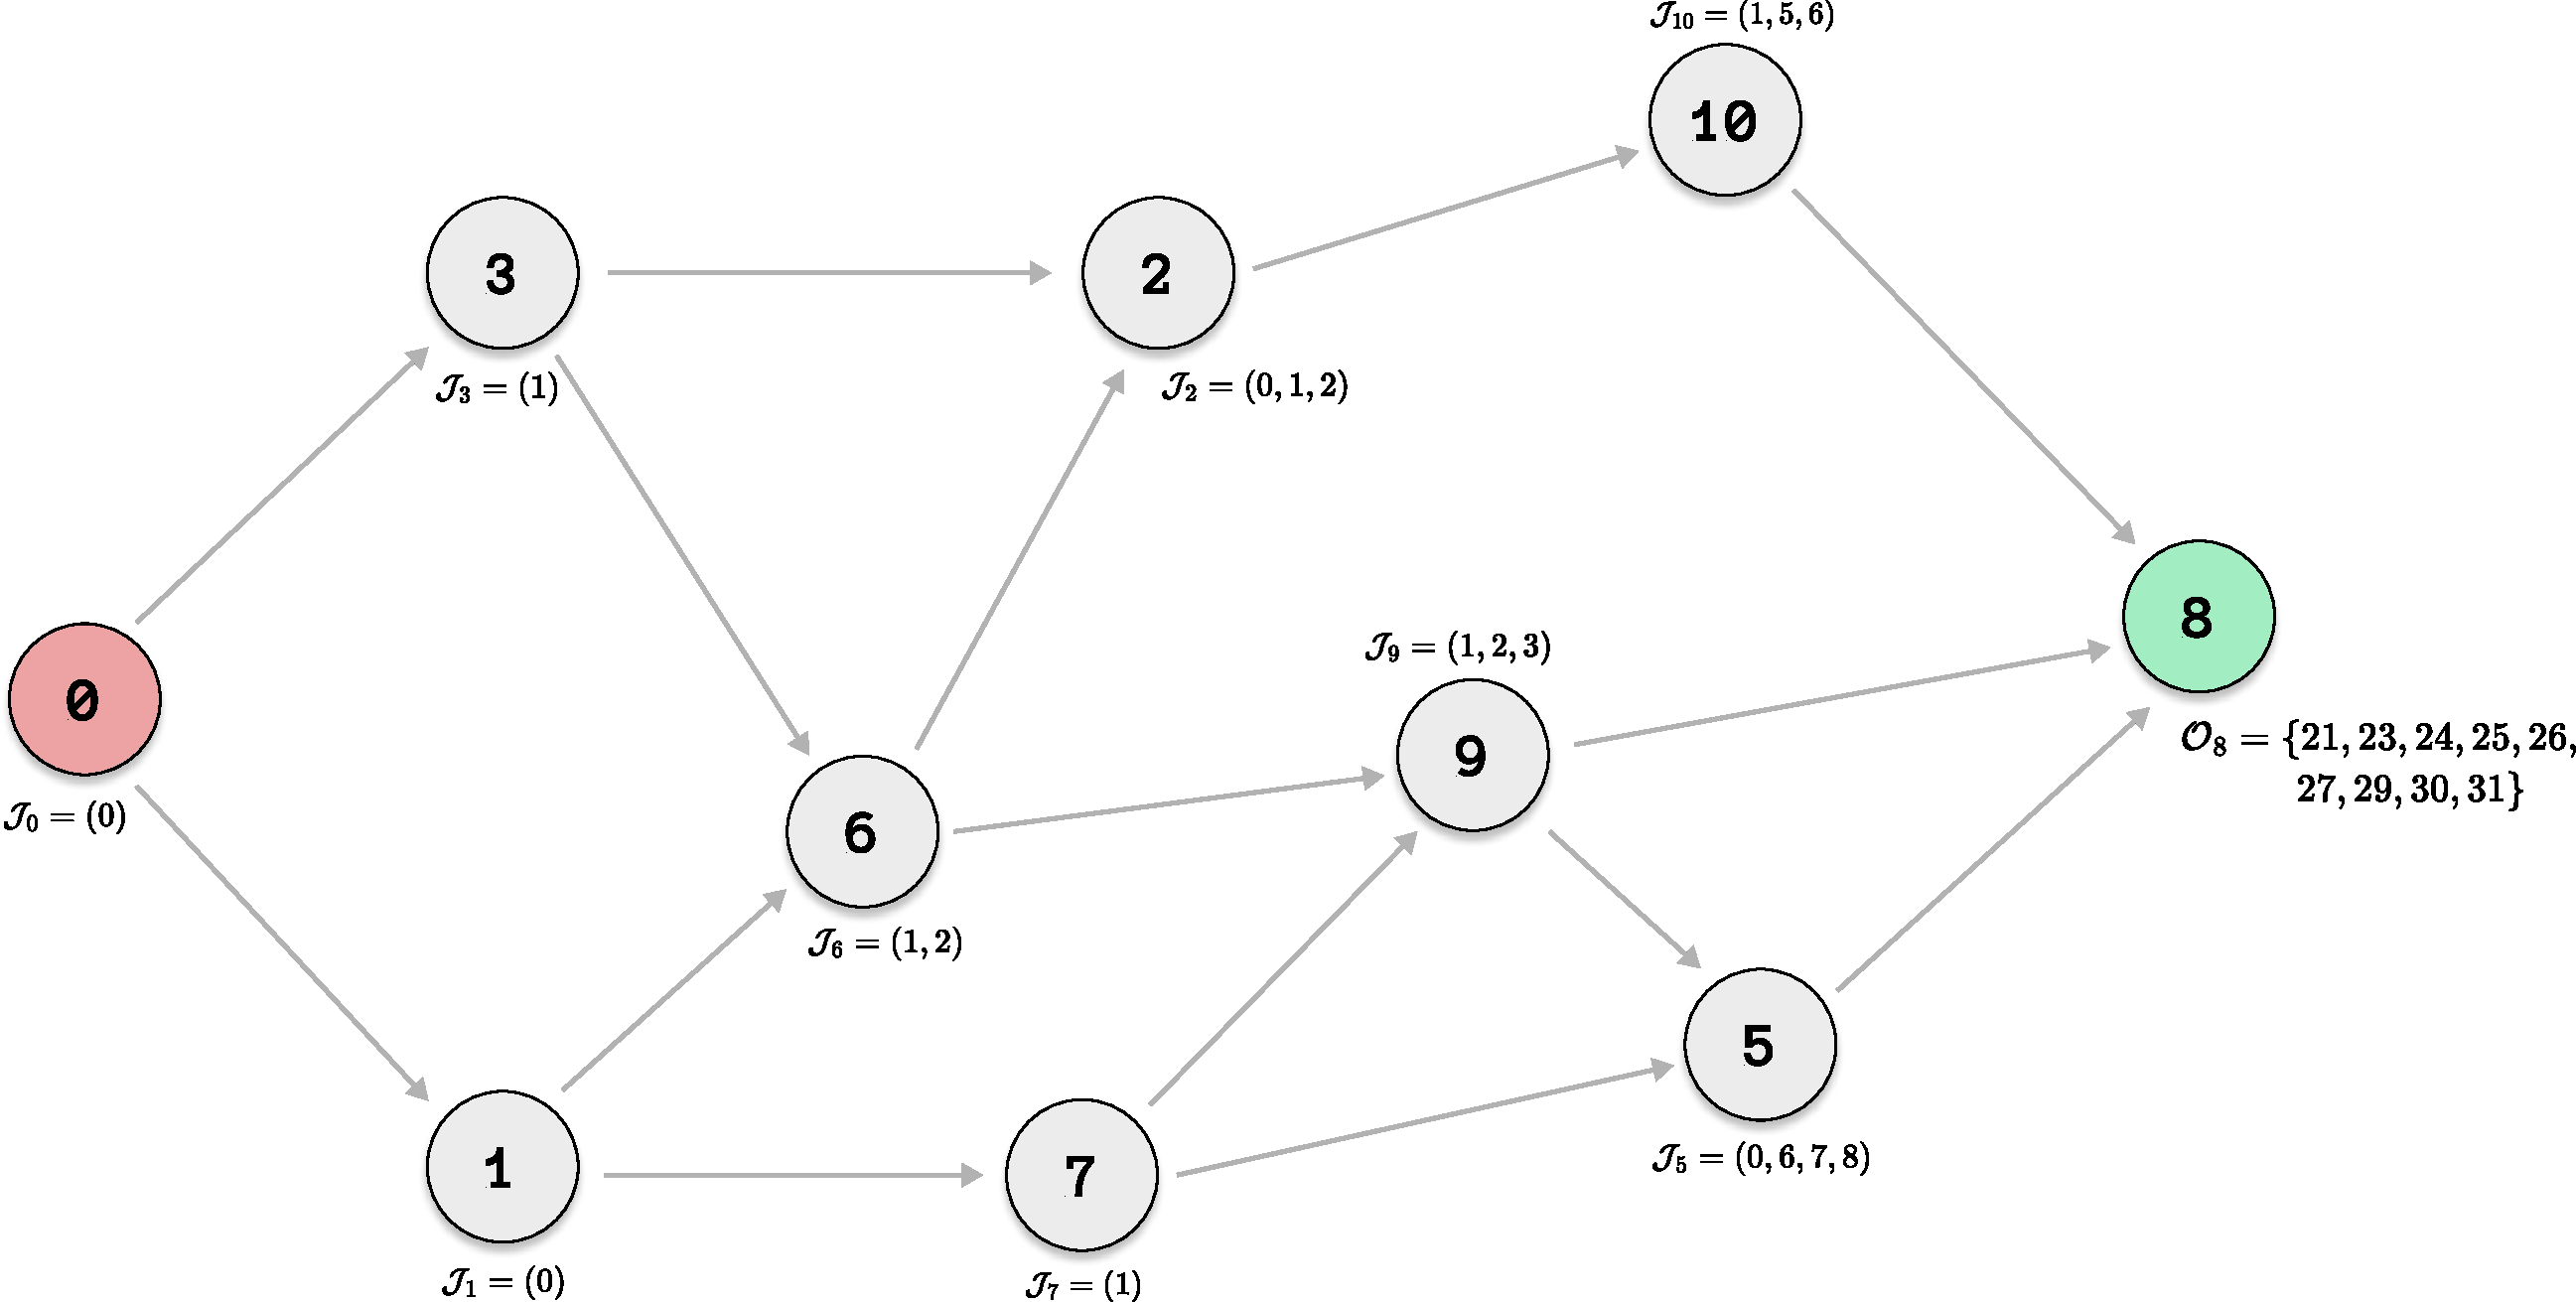
\includegraphics[width=0.9\textwidth]{../bachelor-thesis/TeX/assets/succinct-dag1.pdf}}
%         \only<2>{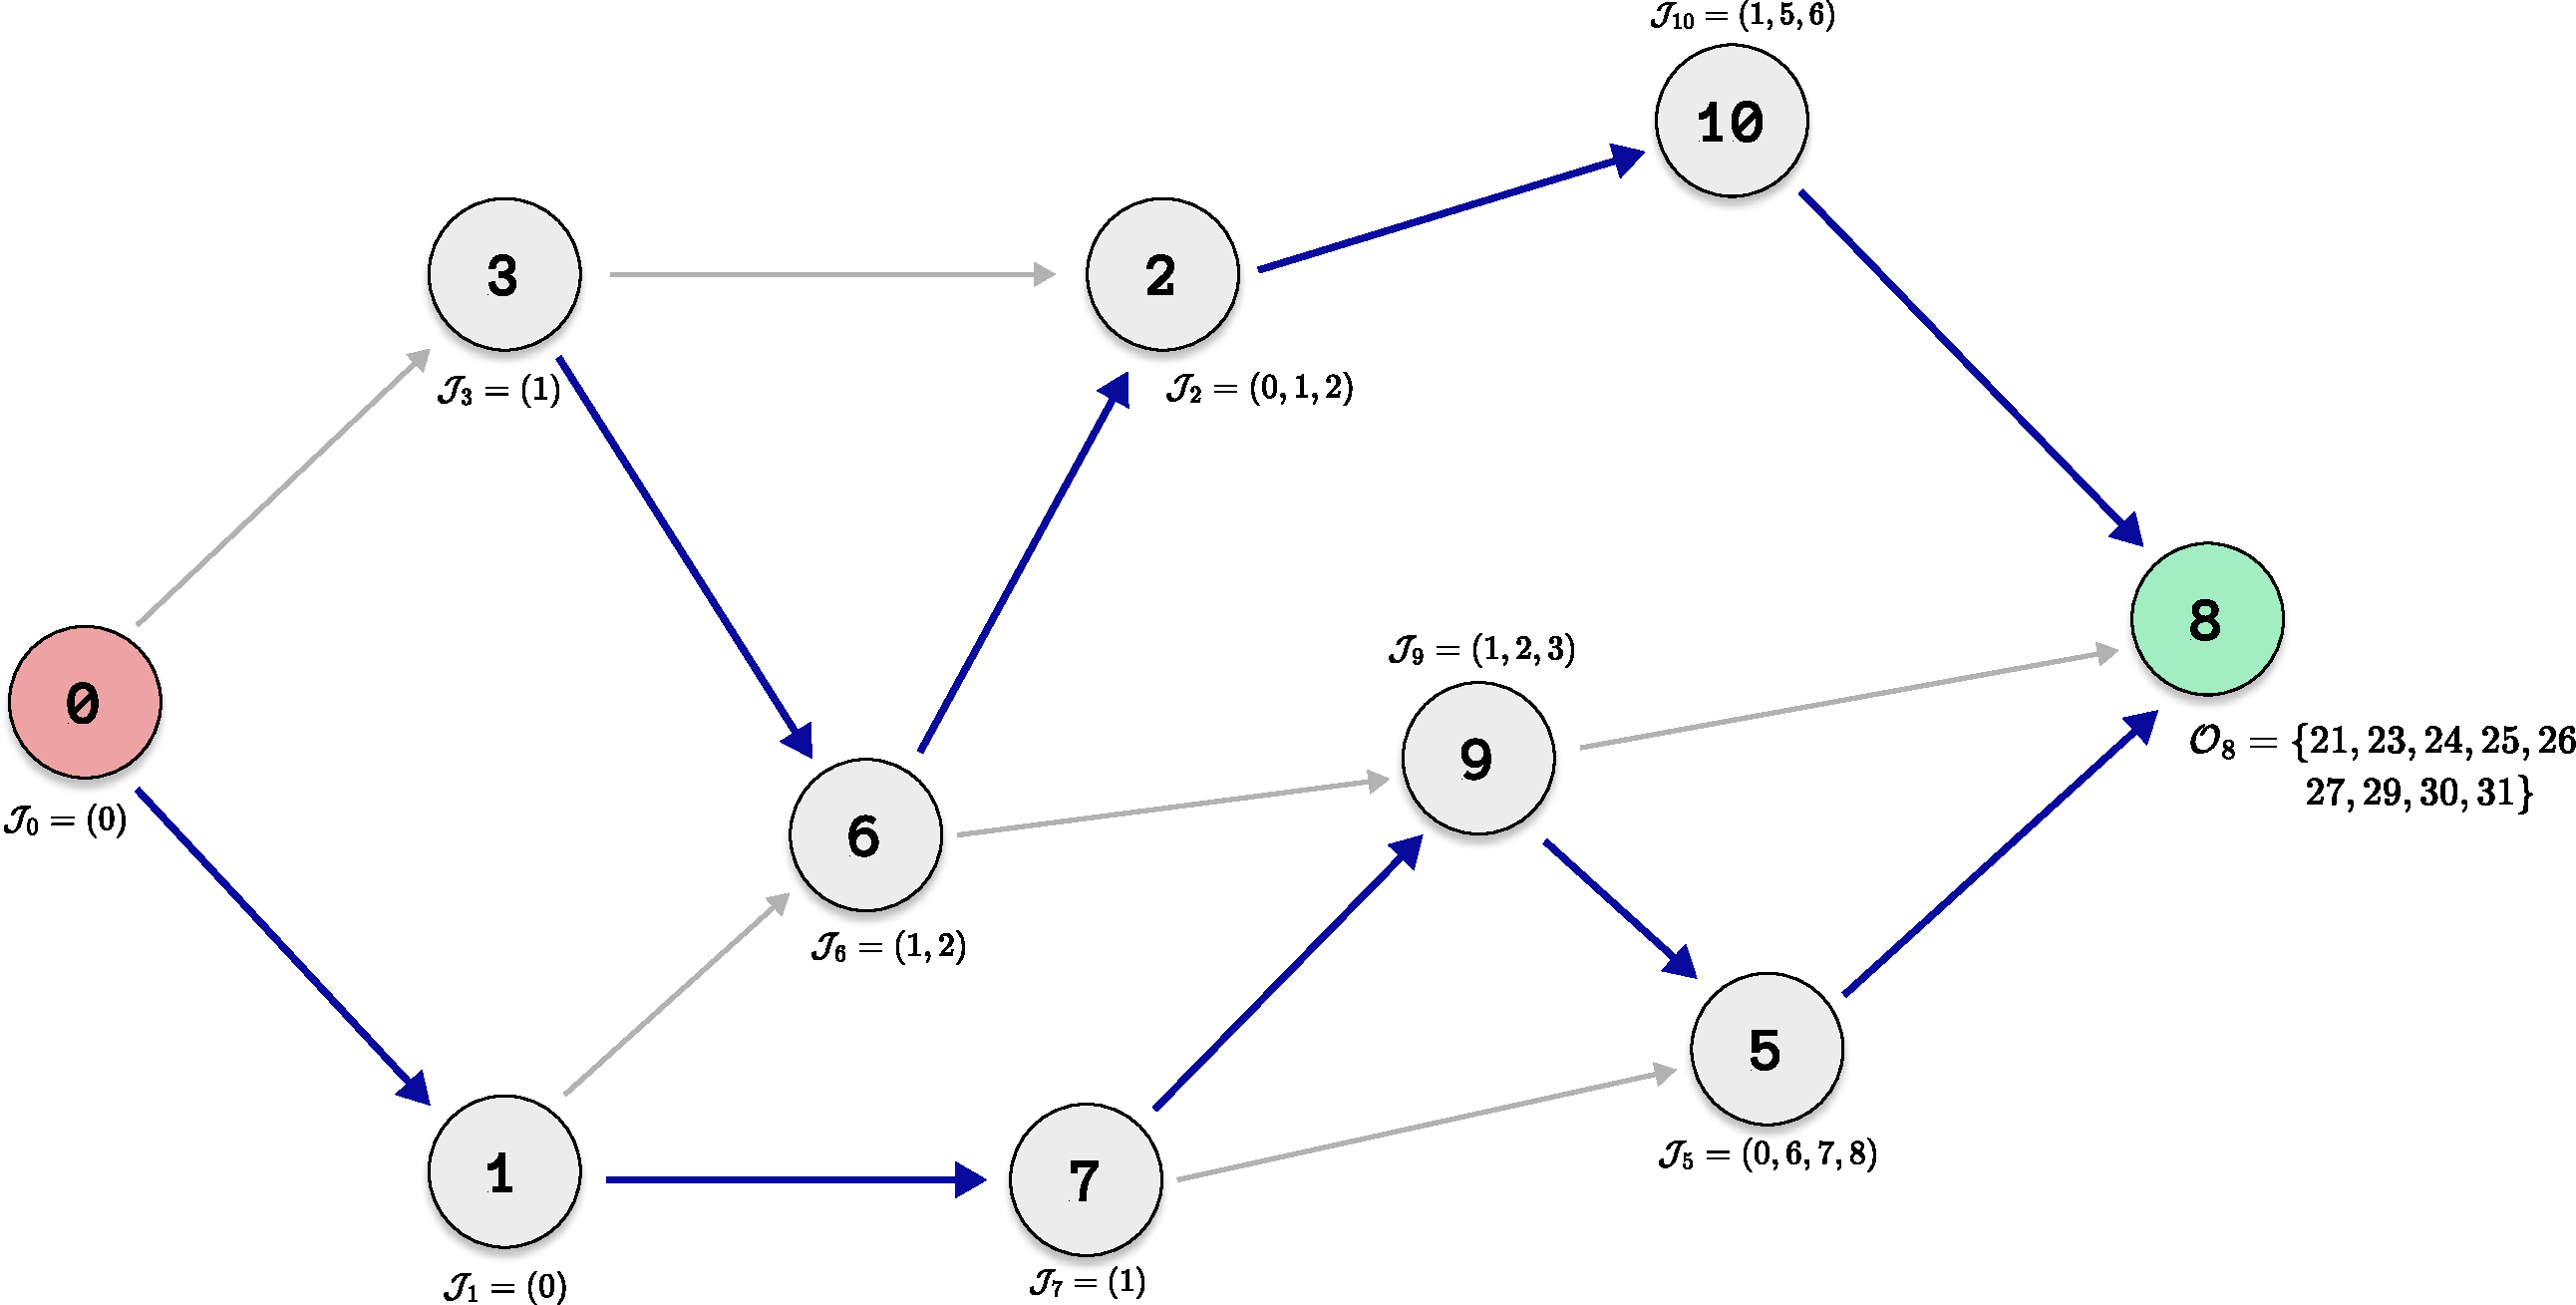
\includegraphics[width=0.9\textwidth]{../bachelor-thesis/TeX/assets/succinct-dag2.pdf}}
%     \end{figure}
% \end{frame}

% --- SLIDE 17: Example: Computing O_7[0] (Static Structure First) ---
\begin{frame}{Example: Computing $\mathcal{O}_7[0]$}
    \framesubtitle{Following the Successor Path: $7 \to 9 \to 5 \to 8$}
    \begin{figure}[hbtp]
        \centering
        % Replace TikZ with sequential images
        \only<1>{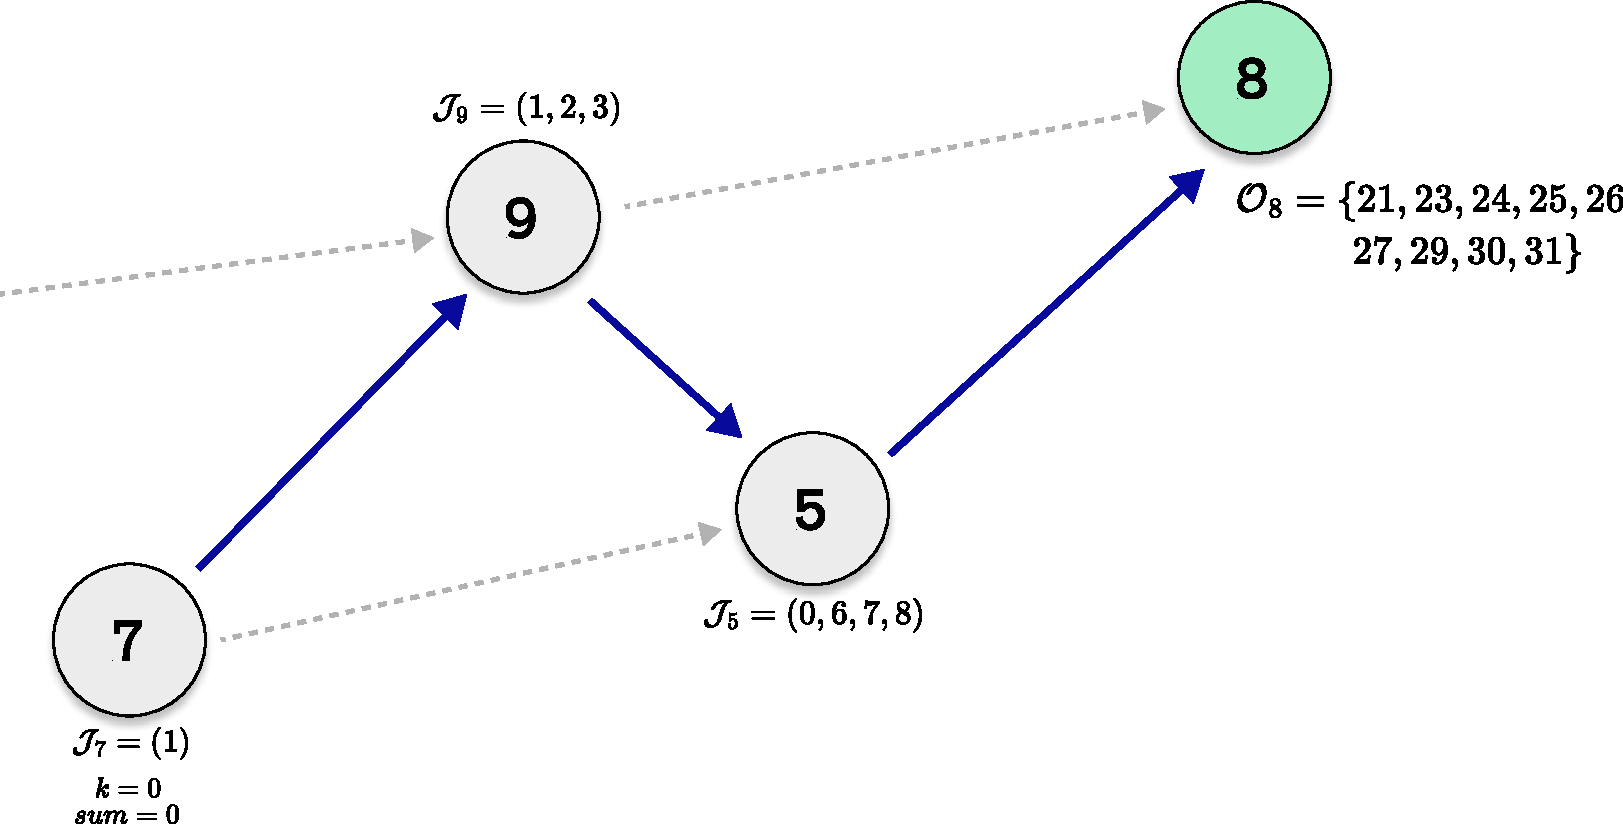
\includegraphics[width=0.9\textwidth]{assets/dag_query1.pdf}}
        \only<2>{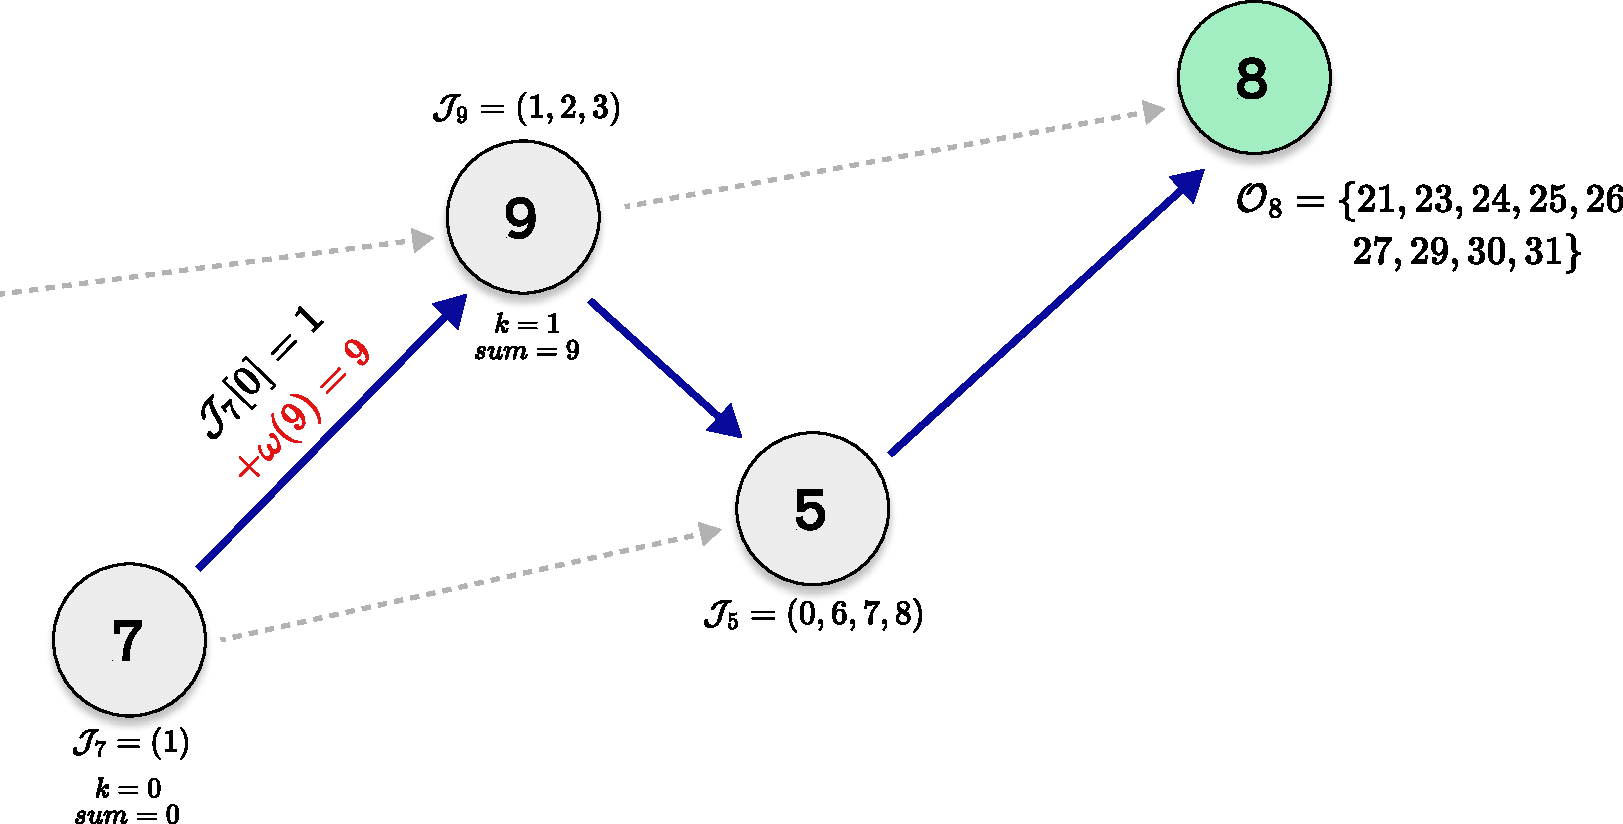
\includegraphics[width=0.9\textwidth]{assets/dag_query2.pdf}}
        \only<3>{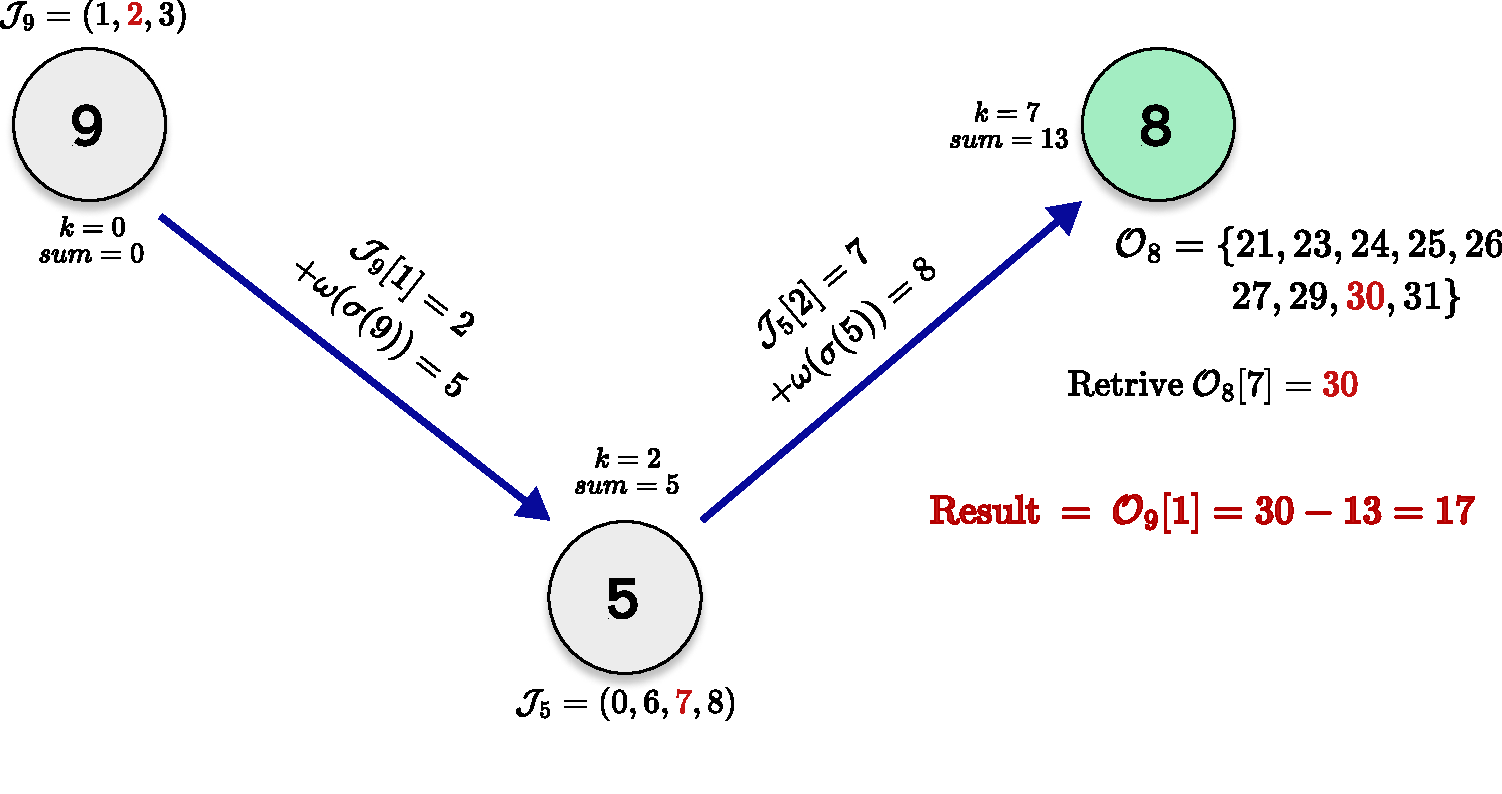
\includegraphics[width=0.9\textwidth]{assets/dag_query3.pdf}}
        \only<4>{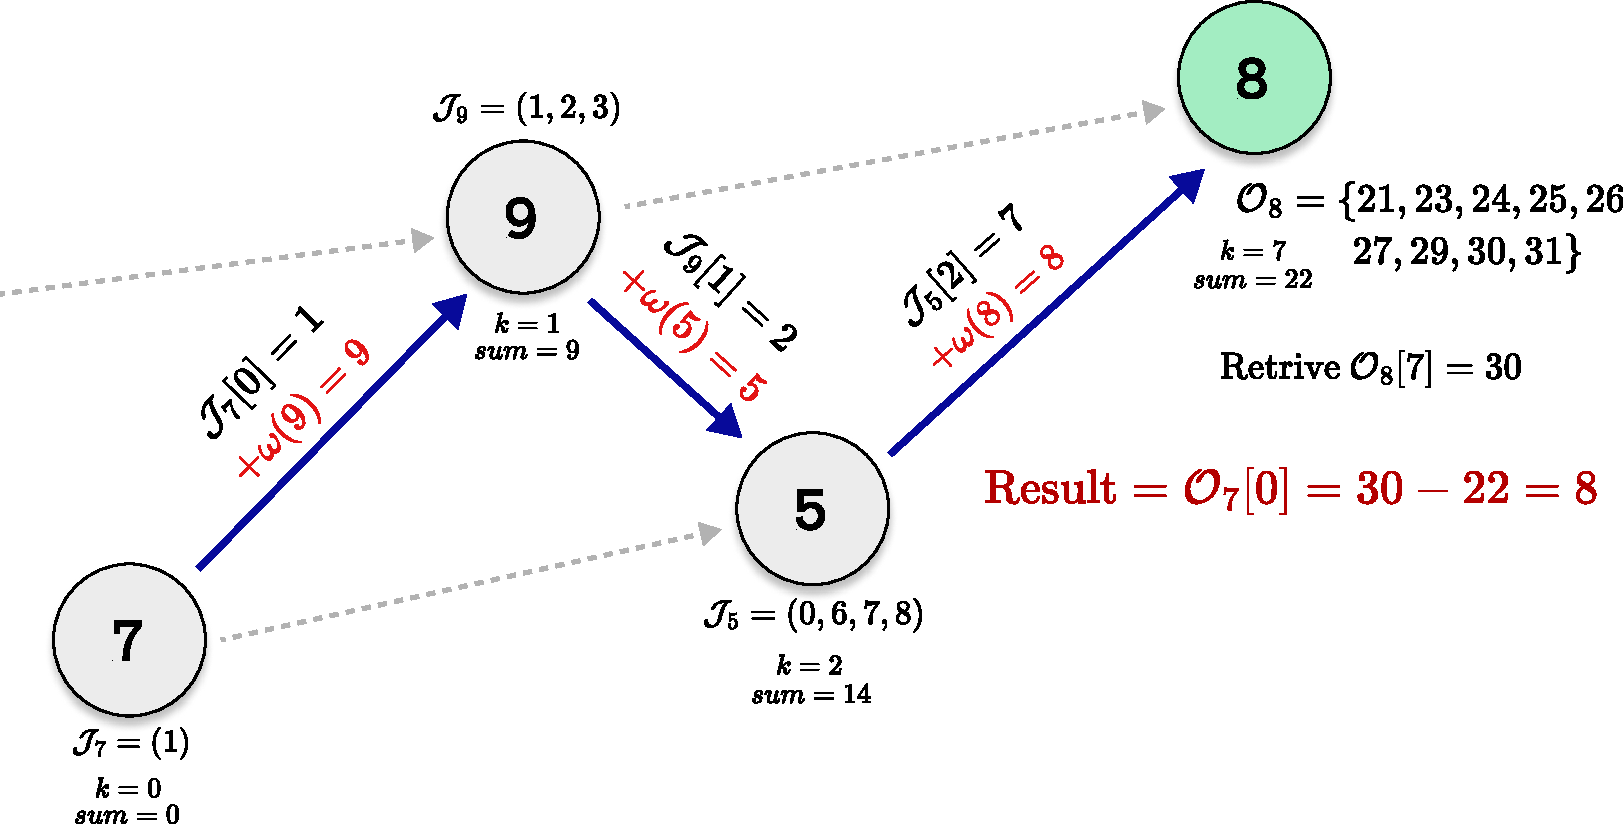
\includegraphics[width=0.9\textwidth]{assets/dag_query4.pdf}}
    \end{figure}
\end{frame}

% --- SLIDE 18: Example: Computing O_7[0] (Dynamic Structure) ---
\begin{frame}{Succinct Data Structure: Components}
    \framesubtitle{Arrays Indexed by Vertex ID}
    % divide in two columns
    \begin{columns}[T]
        \column{0.5\textwidth}
        \uncover<1->{\begin{center}
                \textbf{Each node stores 3 components}
            \end{center}
            \begin{center}
                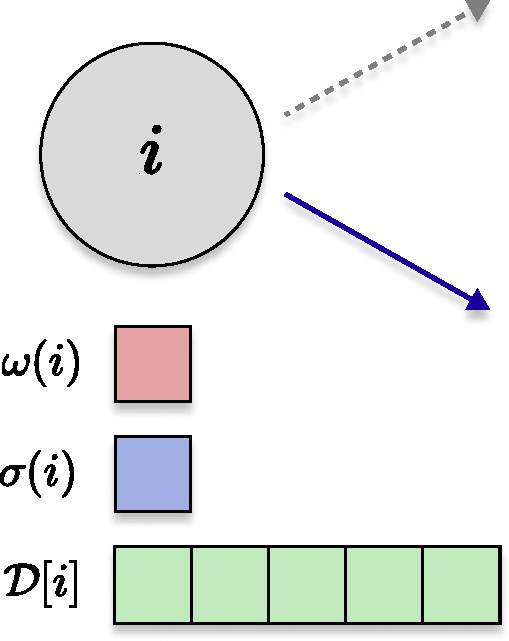
\includegraphics[width=0.55\textwidth]{assets/AoS.pdf}
            \end{center}}

        \column{0.5\textwidth}
        \uncover<2->{\begin{center}
                \textbf{Succinct DAG as a Struct of Arrays}
            \end{center}
            \begin{center}
                \vspace{0.5em}
                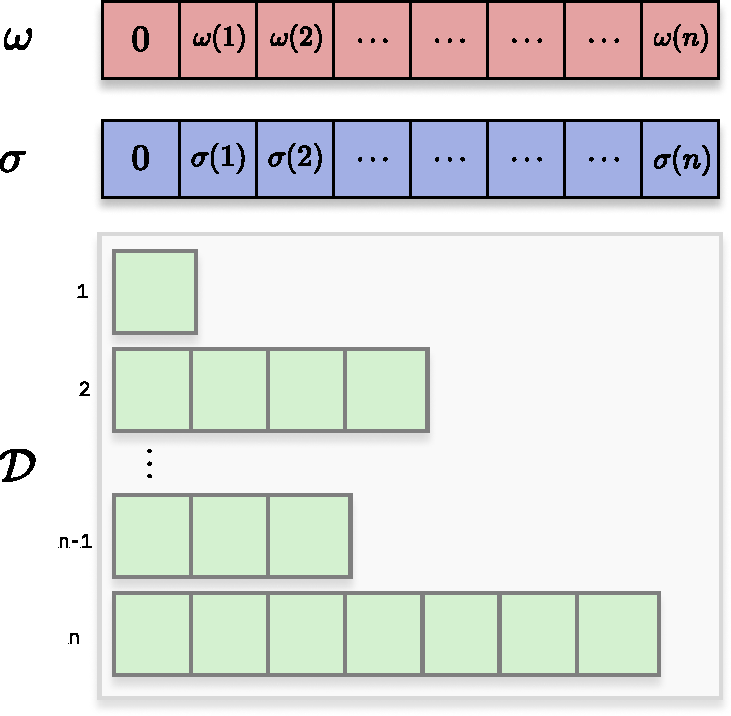
\includegraphics[width=0.8\textwidth]{assets/SoA.pdf}
            \end{center}}
    \end{columns}
\end{frame}
